\chapter{Simulation and Reconstruction}\label{chap:SimReco}
In order to perform physics analysis, measurements made by the ATLAS detector are reconstructed into meaningful physics objects. Offline reconstruction software performs the reconstruction on saved data which passes the trigger selection on the LHC computing grid in several steps. The main reconstruction is handled by \emph{Tier-0} sites, while the creation of compressed sets of data and MC samples are handled by a world-wide network of computing centers.

The reconstruction and identification of the types of physics objects used in the thesis are described in this section. 
\section{Reconstruction of physics objects}

\subsection{Tracks and vertex reconstruction}\label{sec:reconstruction:tracks}
The identification of tracks are important in reconstruction of physics objects and to identify vertices. The aim of track reconstruction is to describe the trajectory of a particle through the inner detector. However, for muons tracks are reconstructed also in the muon spectrometer described in ~\cref{sec:method:MS}. A series of sequential algorithms are used to reconstruct tracks from the inner detector readout~\cite{ATLAS:tracking}. 

Measurements from the pixel and SCT layers are reconstructed into \emph{hits}, defined by three dimensional space points. Hits from either side of the modules is required to form both coordinate in the SCT and timing information from the TRT is used to construct drift circles. \emph{Track seeds} are formed from three hits in the pixel detector and the first layer of the SCT. These track seeds are extended into the outmost layers of the SCT to give \emph{track candidates}, which are then fit to hits using a Kalman-filter~\cite{ATLAS:tracking,ATLAS:Kalman}. The Kalman-filter takes into account the scattering of tracks by materials of the detector. Poor quality tracks are rejected by applying a score based on the $\chi^2$ of the fit and number of missing hits in active detector layers. Ambiguities of space points corresponding to multiple tracks are also removed by selecting the highest scoring tracks. The remaining tracks are then extended to the TRT to provide many more additional hits. Final reconstructed tracks are then formed by fitting to all the detector components simultaneously. 

A subsequent algorithm extending inwards from hits in the TRT is used to find track segments that were missed by the previous method. Tracks segments in the TRT not associated with tracks in the first algorithm are extrapolated inwards to hits in the SCT and pixel detectors. An example of such track segments seen in the inner detector is shown in \cref{fig:method:tracking-outside-in}. Similar ambiguity resolving criteria as the first algorithm based on the $\chi^2$ is applied. 
\begin{figure}[]
    \centering
    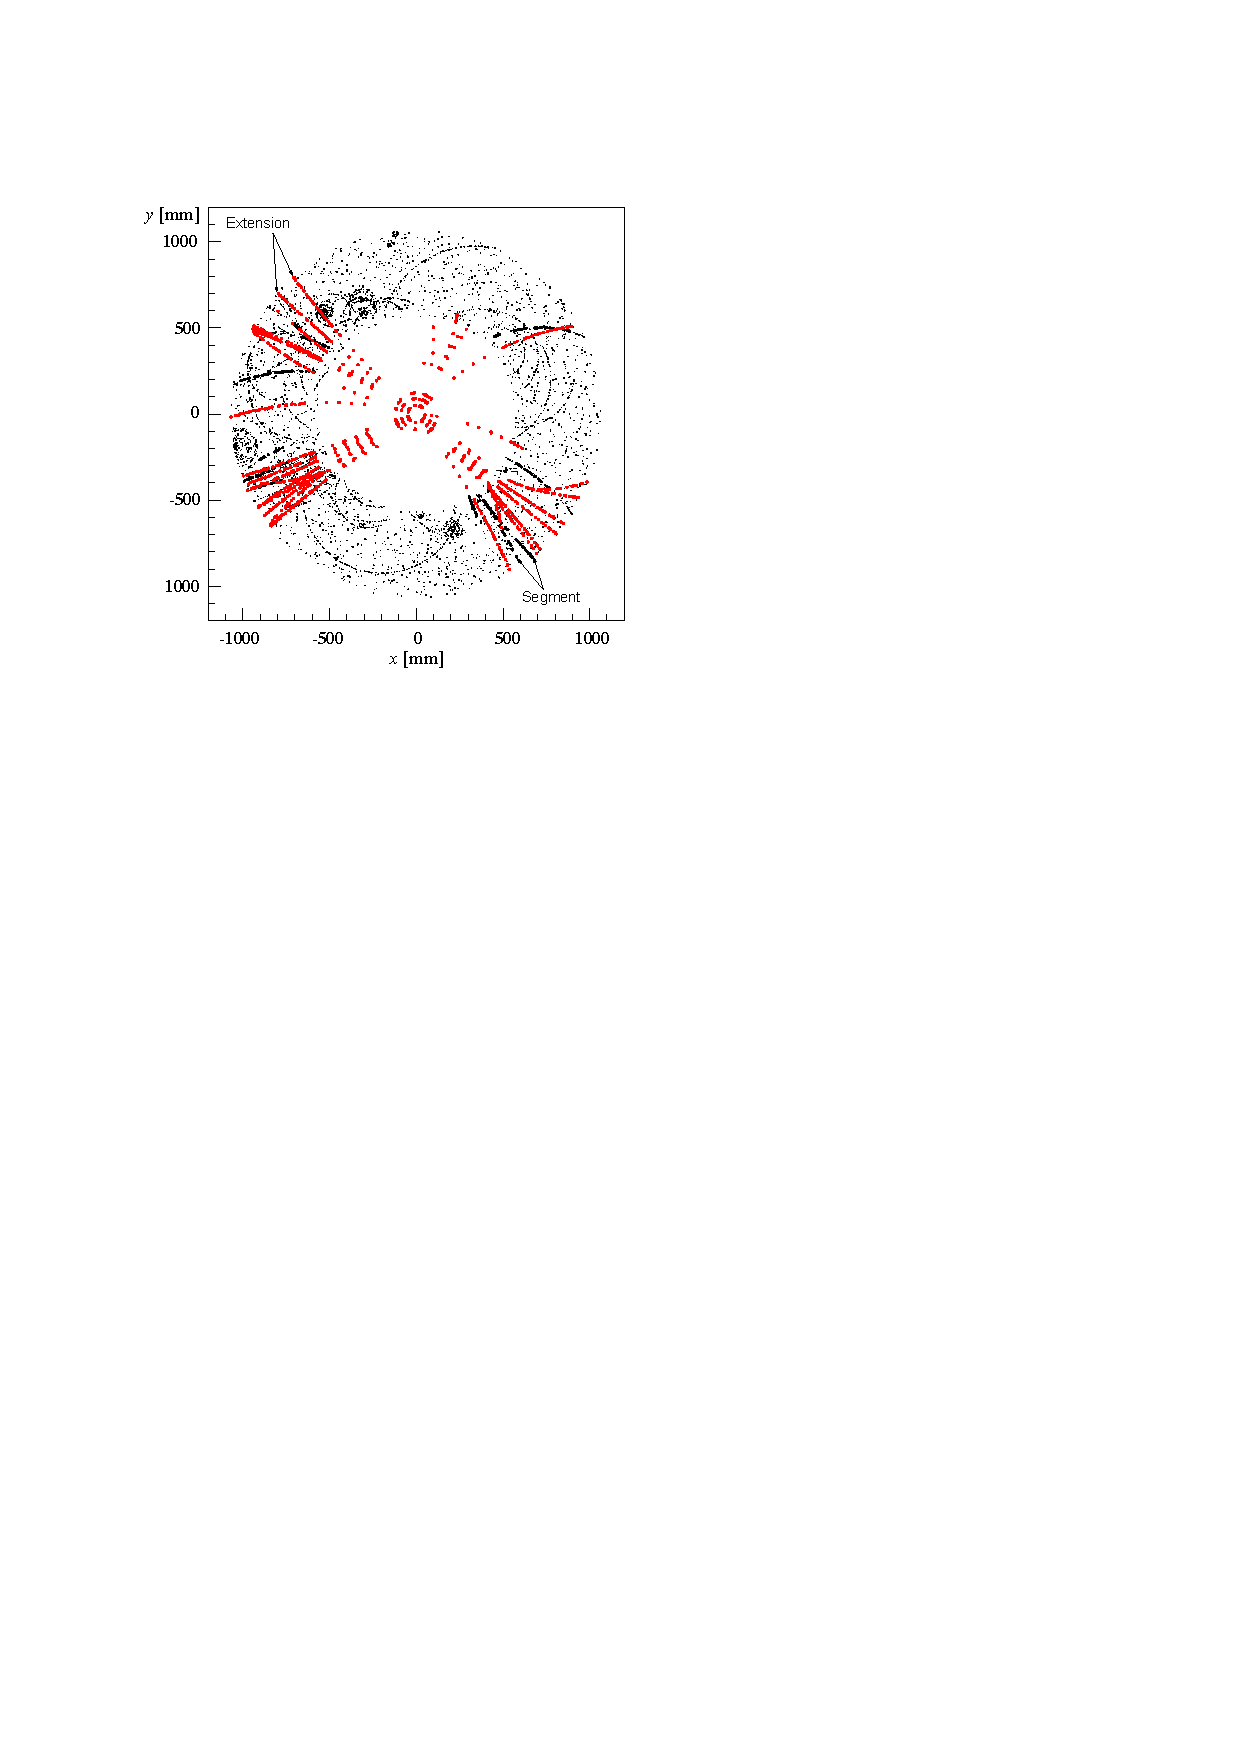
\includegraphics[width=\mediumfigwidth]{images/tracking-outside-in.pdf}
    \caption[Track finding for a simulated \ttbar event]{Track finding for the same simulated \ttbar event.
    Hits are indicated by small black dots in the transverse plane.
    Red dots show hits in associated with tracks that originate from following the SpacePoint seeded tracks into the TRT
    Black circles indicate hits that form track segments in the TRT , which builds the start point of the back tracking application
        From~\cite{ATLAS:tracking}.}
    \label{fig:method:tracking-outside-in}
\end{figure}

There are multiple \emph{pp} collisions per bunch crossing at the LHC due to it's high instantaneous luminosity. \cref{fig:method:ATLAS-pileup} shows the distribution of the number of interactions per bunch crossing. A vertex of an interaction indicates the location in which the physical process has occurred. Once all tracks have been fitted, vertex finder algorithms are used to assign the tracks to their corresponding vertex. Reconstructed vertices are required to have at least two tracks associated with it. The primary vertex is determined as the \emph{pp} interaction vertex with the highest sum of transverse momentum of it's associated tracks, indicating it as the vertex in which the hard scattering is most likely to have originated from. The other \emph{pp}interactions are referred to as \emph{pile up}. Vertex reconstruction is important in removing objects that originate from pileup interactions and for measurements of properties of long lived particles.  
\begin{figure}[]
    \centering
    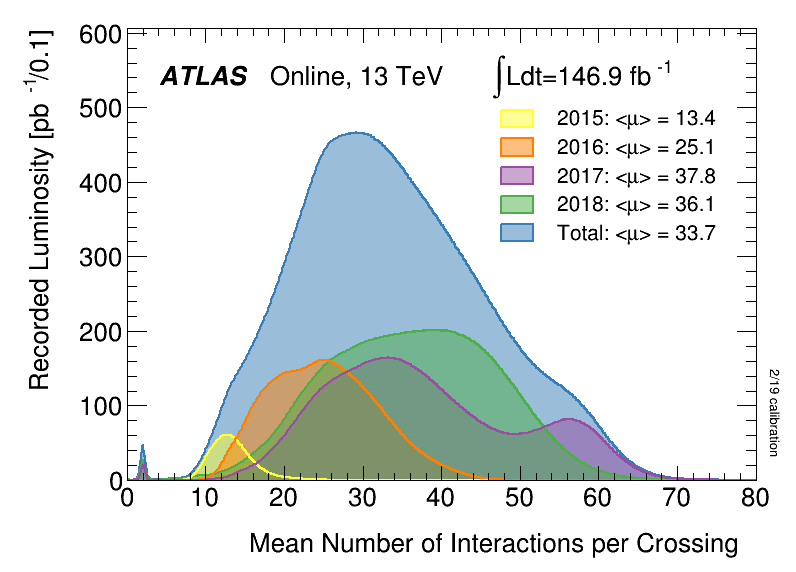
\includegraphics[width=\mediumfigwidth]{images/mu_2015_2018.png}
    \caption[Distribution of number of interactions per \protonproton bunch crossing in ATLAS for the 2015+2018 data-taking period]{Distribution of number of interactions per \protonproton bunch crossing in ATLAS for the 2015+2018 data-taking period.~\cite{ATLAS:lumiPlots}}
    \label{fig:method:ATLAS-pileup}
\end{figure}

\subsection{Electrons}\label{sec:reconstruction:electrons}
Electrons and positrons have the same experimental signature in the EM calorimeter. They are only distinguishable due to the difference in the curvature of their tracks in the ID. In this thesis, positrons will also be denoted as electrons. 

Electron reconstruction involves using track information from the ID with calorimeter information from the EM calorimeter and the pattern of electrons transition radiation as they pass through the TRT.

\subsubsection{Electron reconstruction}
The measurement of an electron signature can be characterised by a localised energy deposit (cluster) in the EM calorimeter followed by charged tracks in the ID that can be matched to the cluster that will form the final electron candidate. Electrons can lose significant energy when traversing the ID due to bremsstrahlung, resulting in radiated photons. These photons can then be converted into electrons which can undergo further bremsstrahlung. Most of then energy of the electrons and photons are deposited within the EM calorimeter as they are collimated. This effect can result in multiple tracks being matched to the same electromagnetic cluster. 

A sliding window algorithm~\cite{slidingwindow} is utilised to search for localised clusters in the EM calorimeter. The EM calorimeter is divided into an $\eta \times \phi$ matrix. Initially windows which correspond to a $3 \times 5$ granularity in the second layer of the EM calorimeter ($0.025 \times 0.025$) are formed. These search the matrix for energy deposits with $E_T > \SI{2.5}{\giga\electronvolt}$. The identified clusters are as seeds to match corresponding reconstructed tracks in the ID. The Gaussian Sum Filter (GSF) method~\cite{ATLAS:CONF-2012-047} is used to refit the reconstructed tracks, which takes into account the effects bremsstrahlung energy loss characteristic to electrons. If no suitable GSF-track is matched to an EM calorimeter cluster, these are labeled as unconverted photons. A converted photon is defined as a photon where the process $Z \rightarrow e^+e^-$ occurs before reaching the EM calorimeter, resulting in a GSF candidate but is not associated with the primary vertex. After matching the track, the cluster is then rebuilt summing the energies of all the cells within the $3 \times 7$ ($5 \times 5$) window in the barrel (end-cap), allowing to account for radiation losses due to bremsstrahlung. 

Using the sliding window algorithm, the efficiency to reconstruct EM-cluster candidates in the EM calorimeter varies as a function of $\eta$ and $E_T$. \cref{fig:method:slidingwindow-reco} shows that the reconstruction efficiency as a function of $E_T$, it ranges from 65\% at $E_T = \SI{4.5}{\giga\electronvolt}$ to more than 99\% above $E_T = \SI{15}{\giga\electronvolt}$. This efficiency is entirely determined from simulation.

\begin{figure}[]
    \centering
    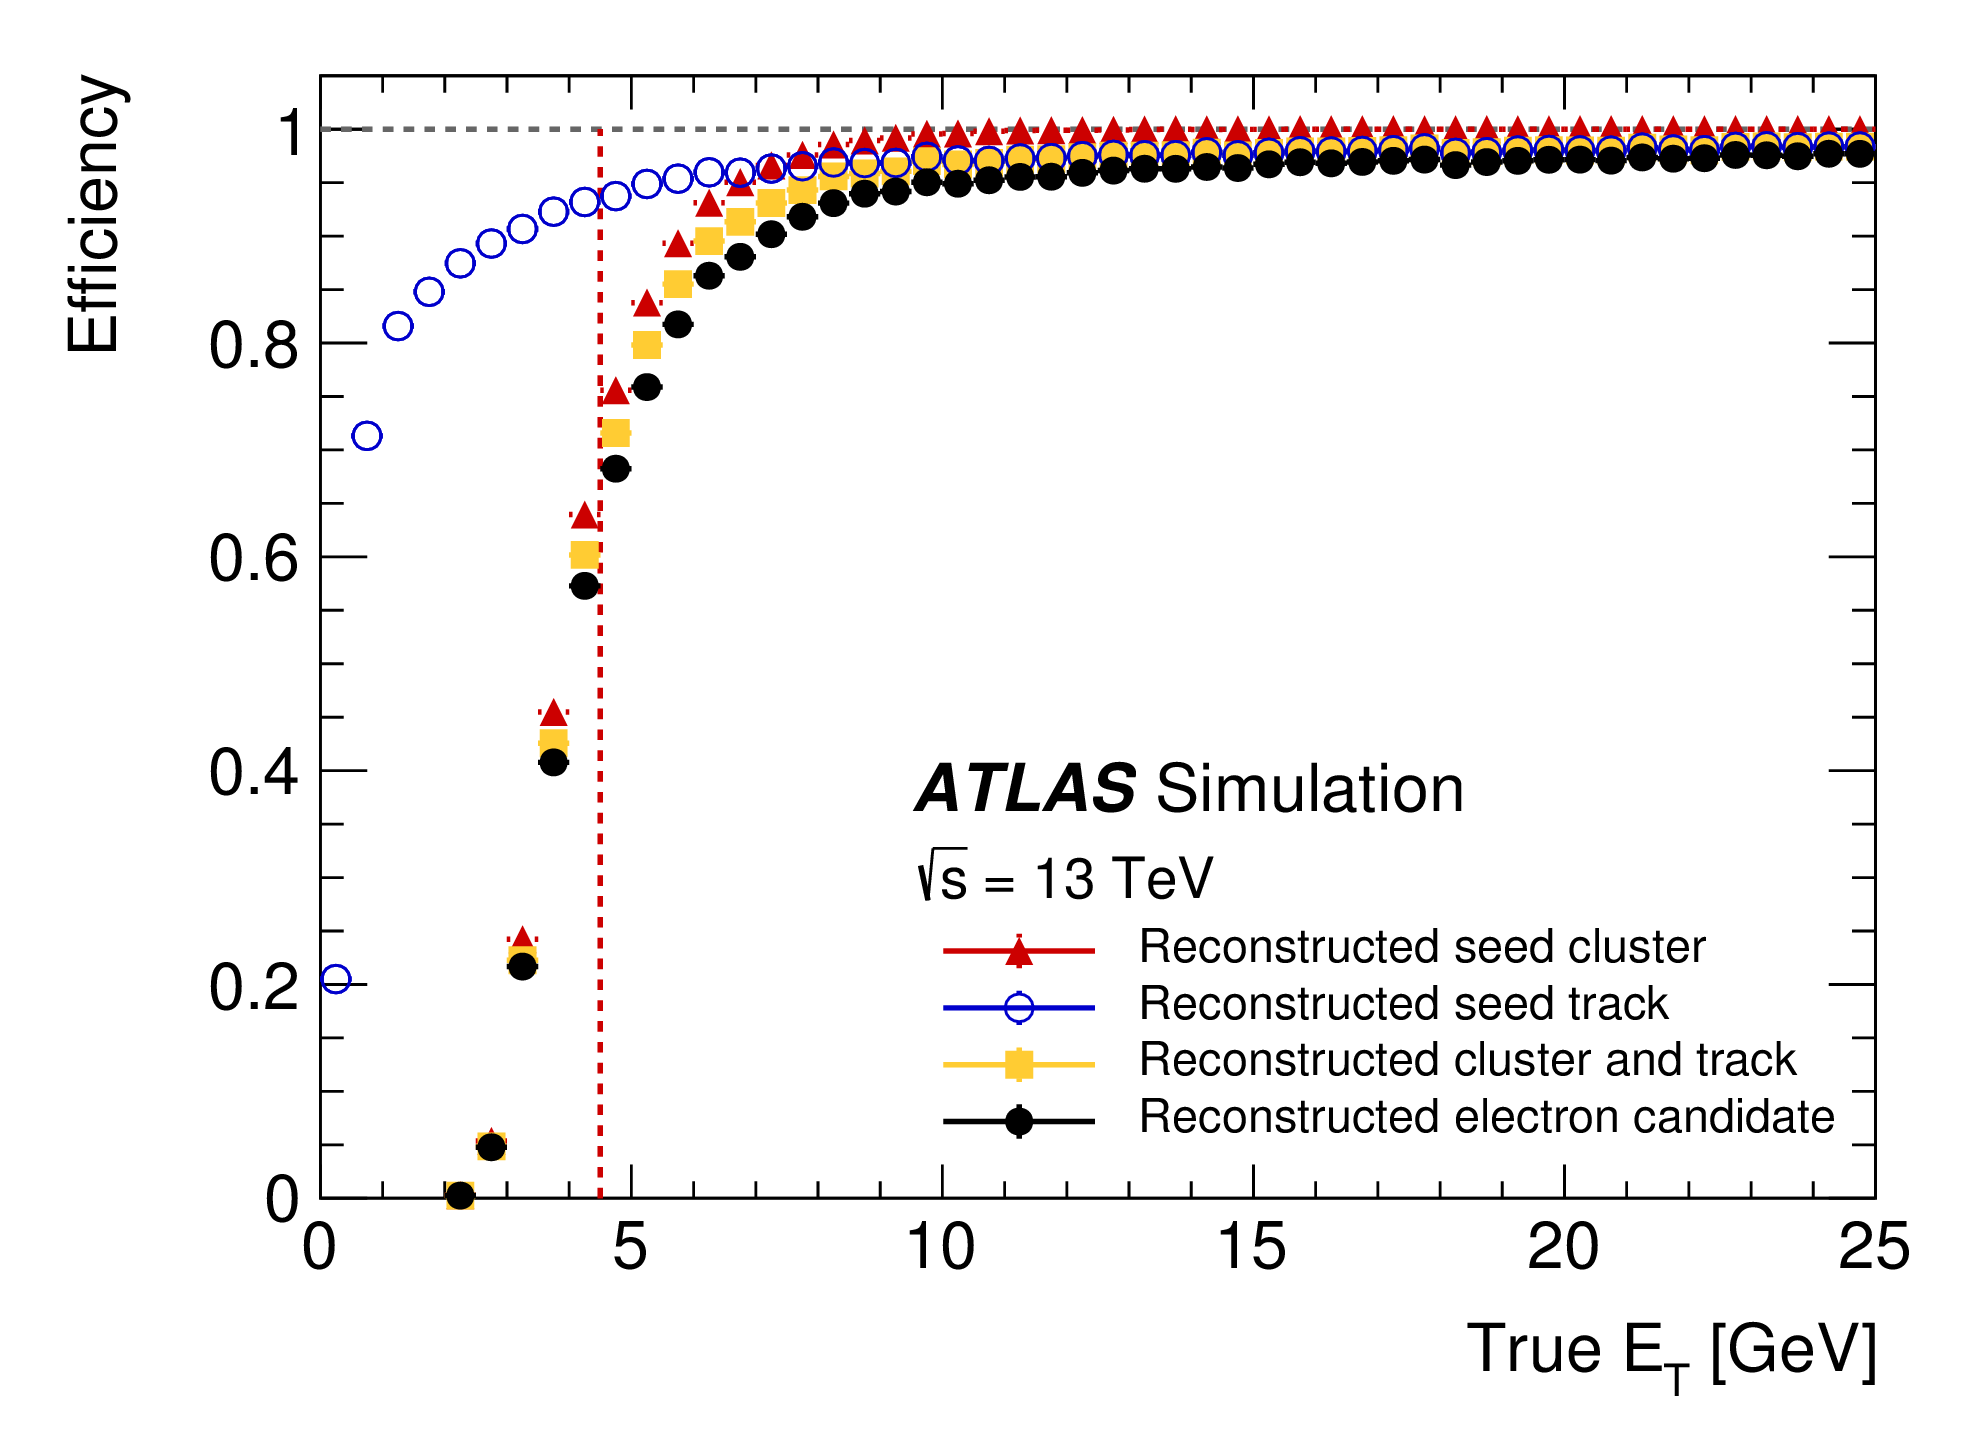
\includegraphics[width=\mediumfigwidth]{images/2015_2016_recoeff.png}
    \caption[Total reconstruction energy for simulated electrons using the sliding window algorithm]{The total reconstruction efficiency for simulated electrons in a single-electron sample as a function of truth level transverse energy, $E_T$, for each step of electron candidate formation ~\cite{slidingwindowreco}.}
    \label{fig:method:slidingwindow-reco}
\end{figure}

From 2017 a new clustering algorithm has been adopted based on topological clusters (topo-cluster)~\cite{Aad:2019tso}. The topological clusters allows for recovery low energy deposits from bremsstrahlung photons and associate them to the electron cluster, forming an \emph{supercluster}. ~\cref{fig:method:superclusterscheme} shows a scheme of this procedure. In contrast to the sliding window algorithm the cell significance, $\zeta^{EM}_{cell}$, is responsible for the seeding in a topo-cluster, and is defined as:

\begin{equation}
    \zeta^{EM}_{cell} = \abs{\frac{E^{EM}_{cell}}{\sigma^{EM}_{cell,noise}}},
\end{equation}

where $\abs{E^{EM}_{cell}}$ is the absolute cell energy and $\sigma^{EM}_{cell,noise}$ is the expected cell noise. The clustering algorithm initially forms a \emph{proto-cluster} using a set of noise thresholds in which the initial cell is required to have $\abs{E^{EM}_{cell}} \geq 4$. Then all immediate neighboring cells with $\abs{E^{EM}_{cell}} \geq 2$ around the proto-cluster are added. Finally, cells with $\abs{E^{EM}_{cell}} \geq 0$ adjacent to the cells that were previously added are added to the cluster. This formalism is known as "4-2-0" topo-cluster reconstruction.
A supercluster is built from a topo-cluster seed after satellite candidates, possibly emerging from bremsstrahlung radiation, around a seed candidate have been resolved. ~\cref{fig:method:screco} shows the efficiency for the different components of the supercluster based reconstruction. The same track fitting method as in the sliding window algorithm is used to refit the reconstructed tracks.
\begin{figure}[h]
    \centering
    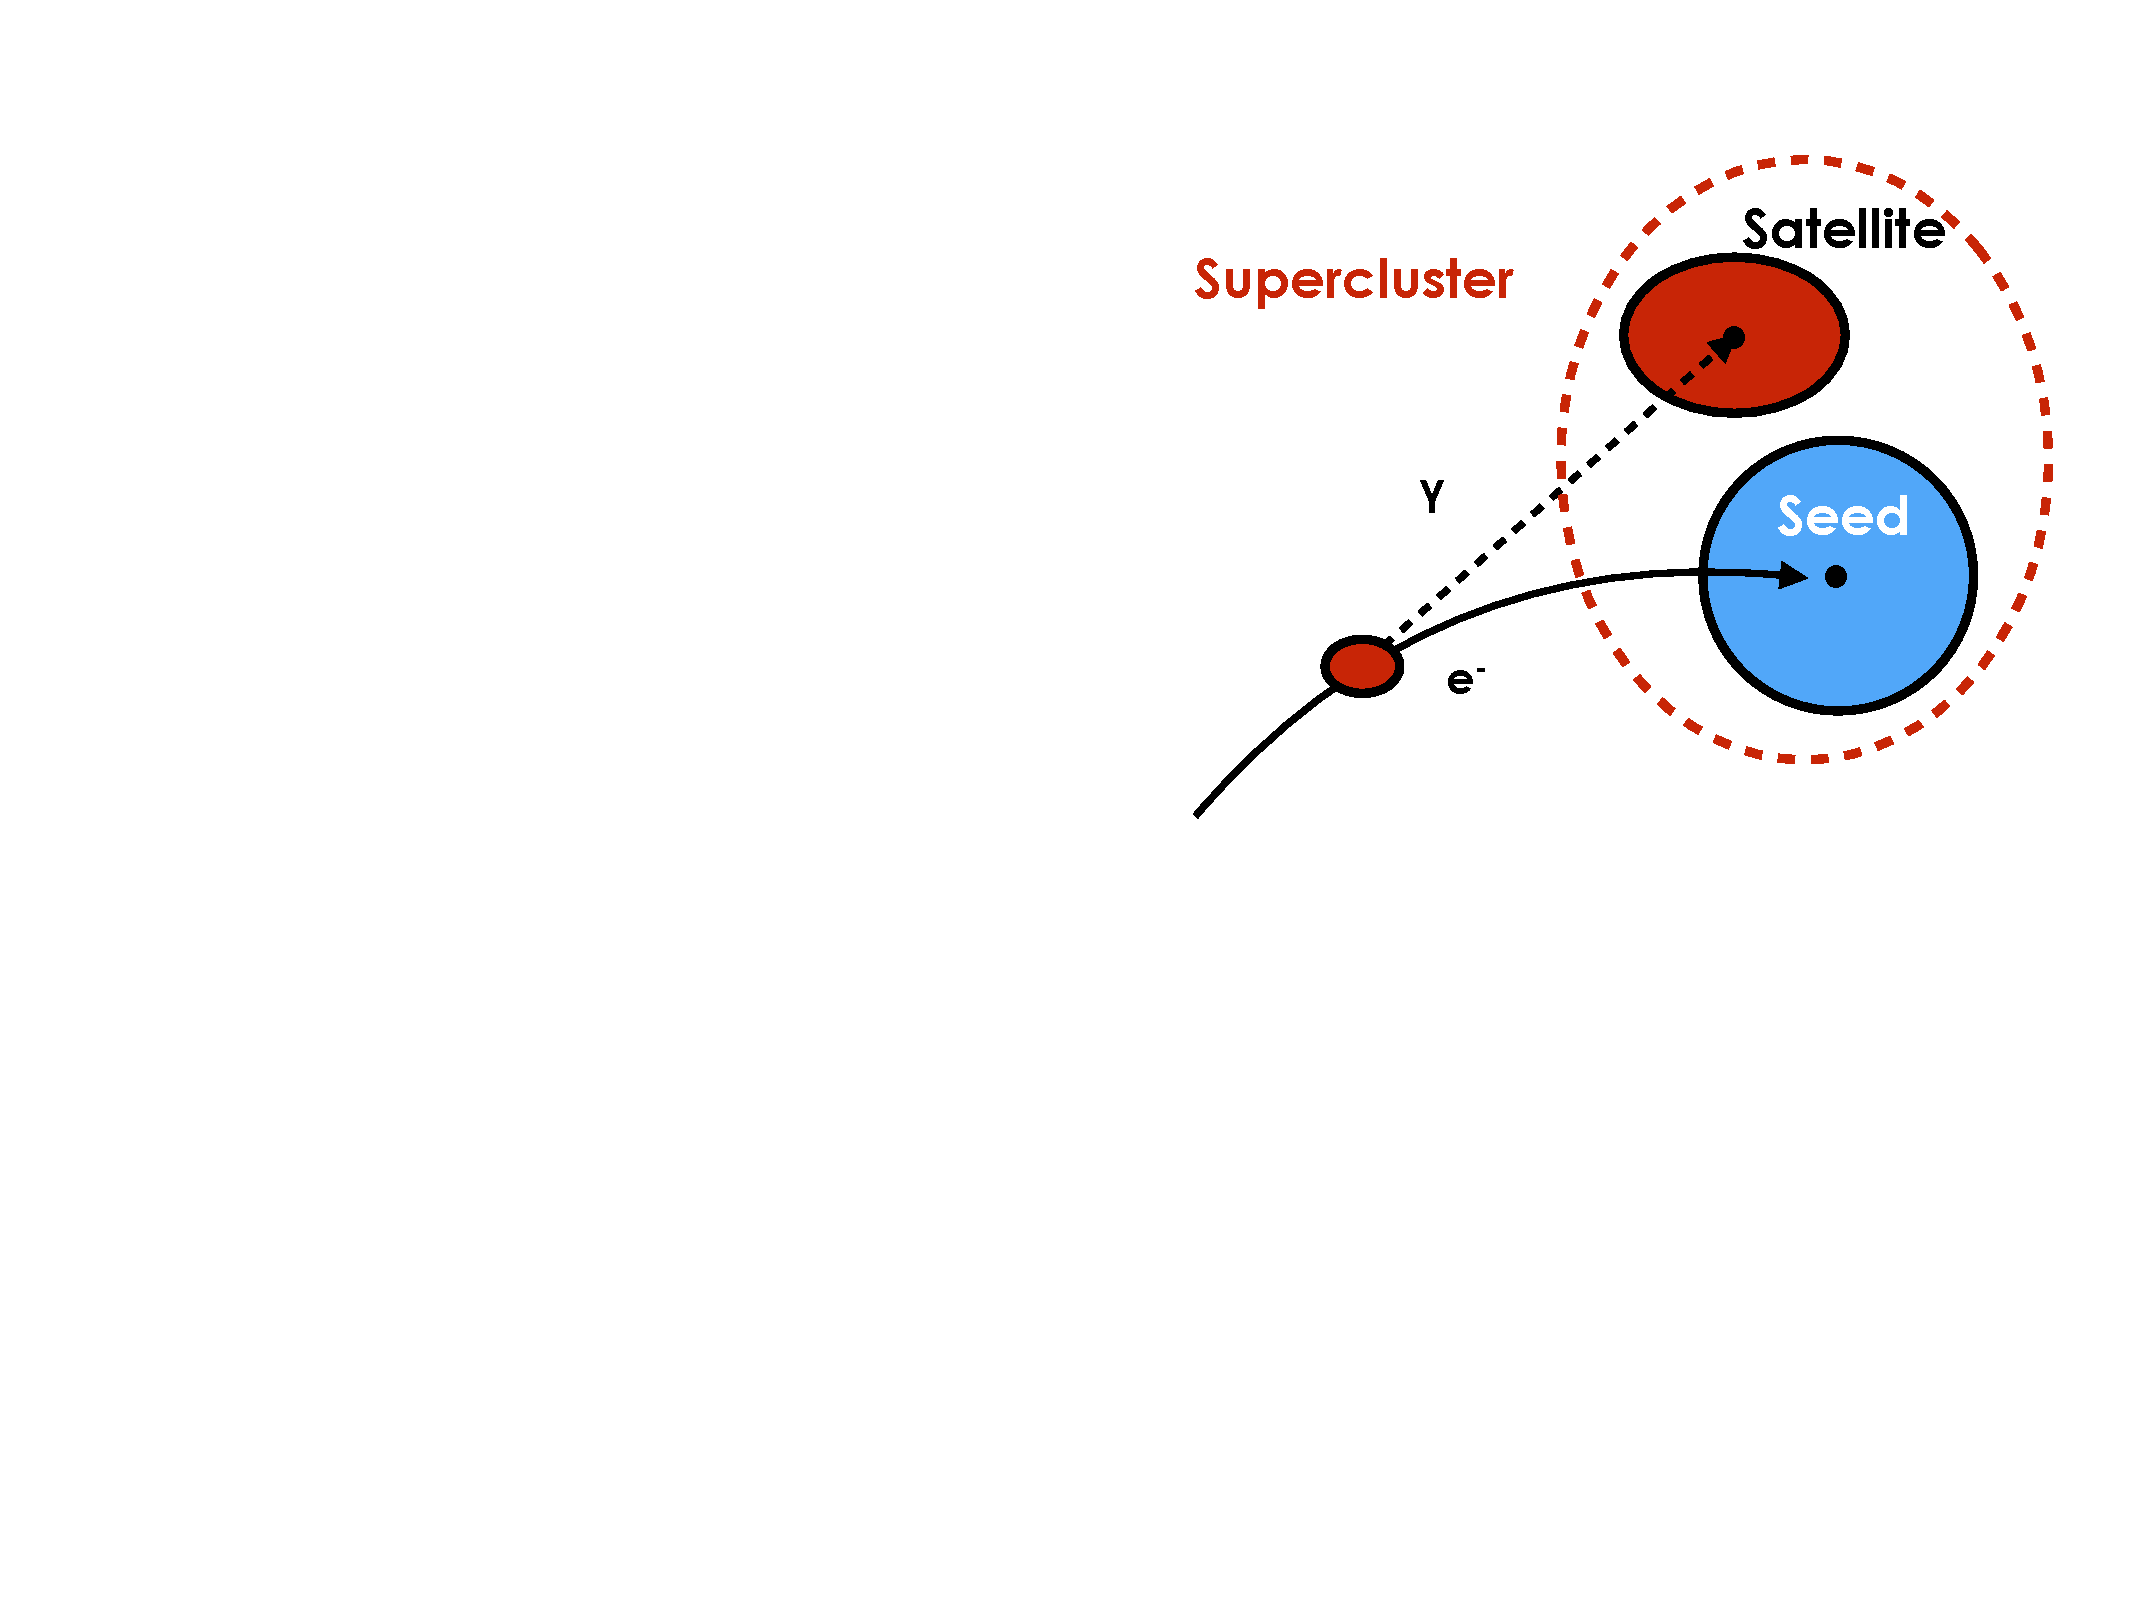
\includegraphics[width=\mediumfigwidth]{images/topo-cluster.pdf}
    \caption[Diagram of an example supercluster showing a seed electron cluster and a satellite photon cluster.]{Diagram of an example supercluster showing a seed electron cluster and a satellite photon cluster ~\cite{ATL-PHYS-PUB-2017-022}.}
    \label{fig:method:superclusterscheme}
\end{figure}
\begin{figure}[h]
    \centering
    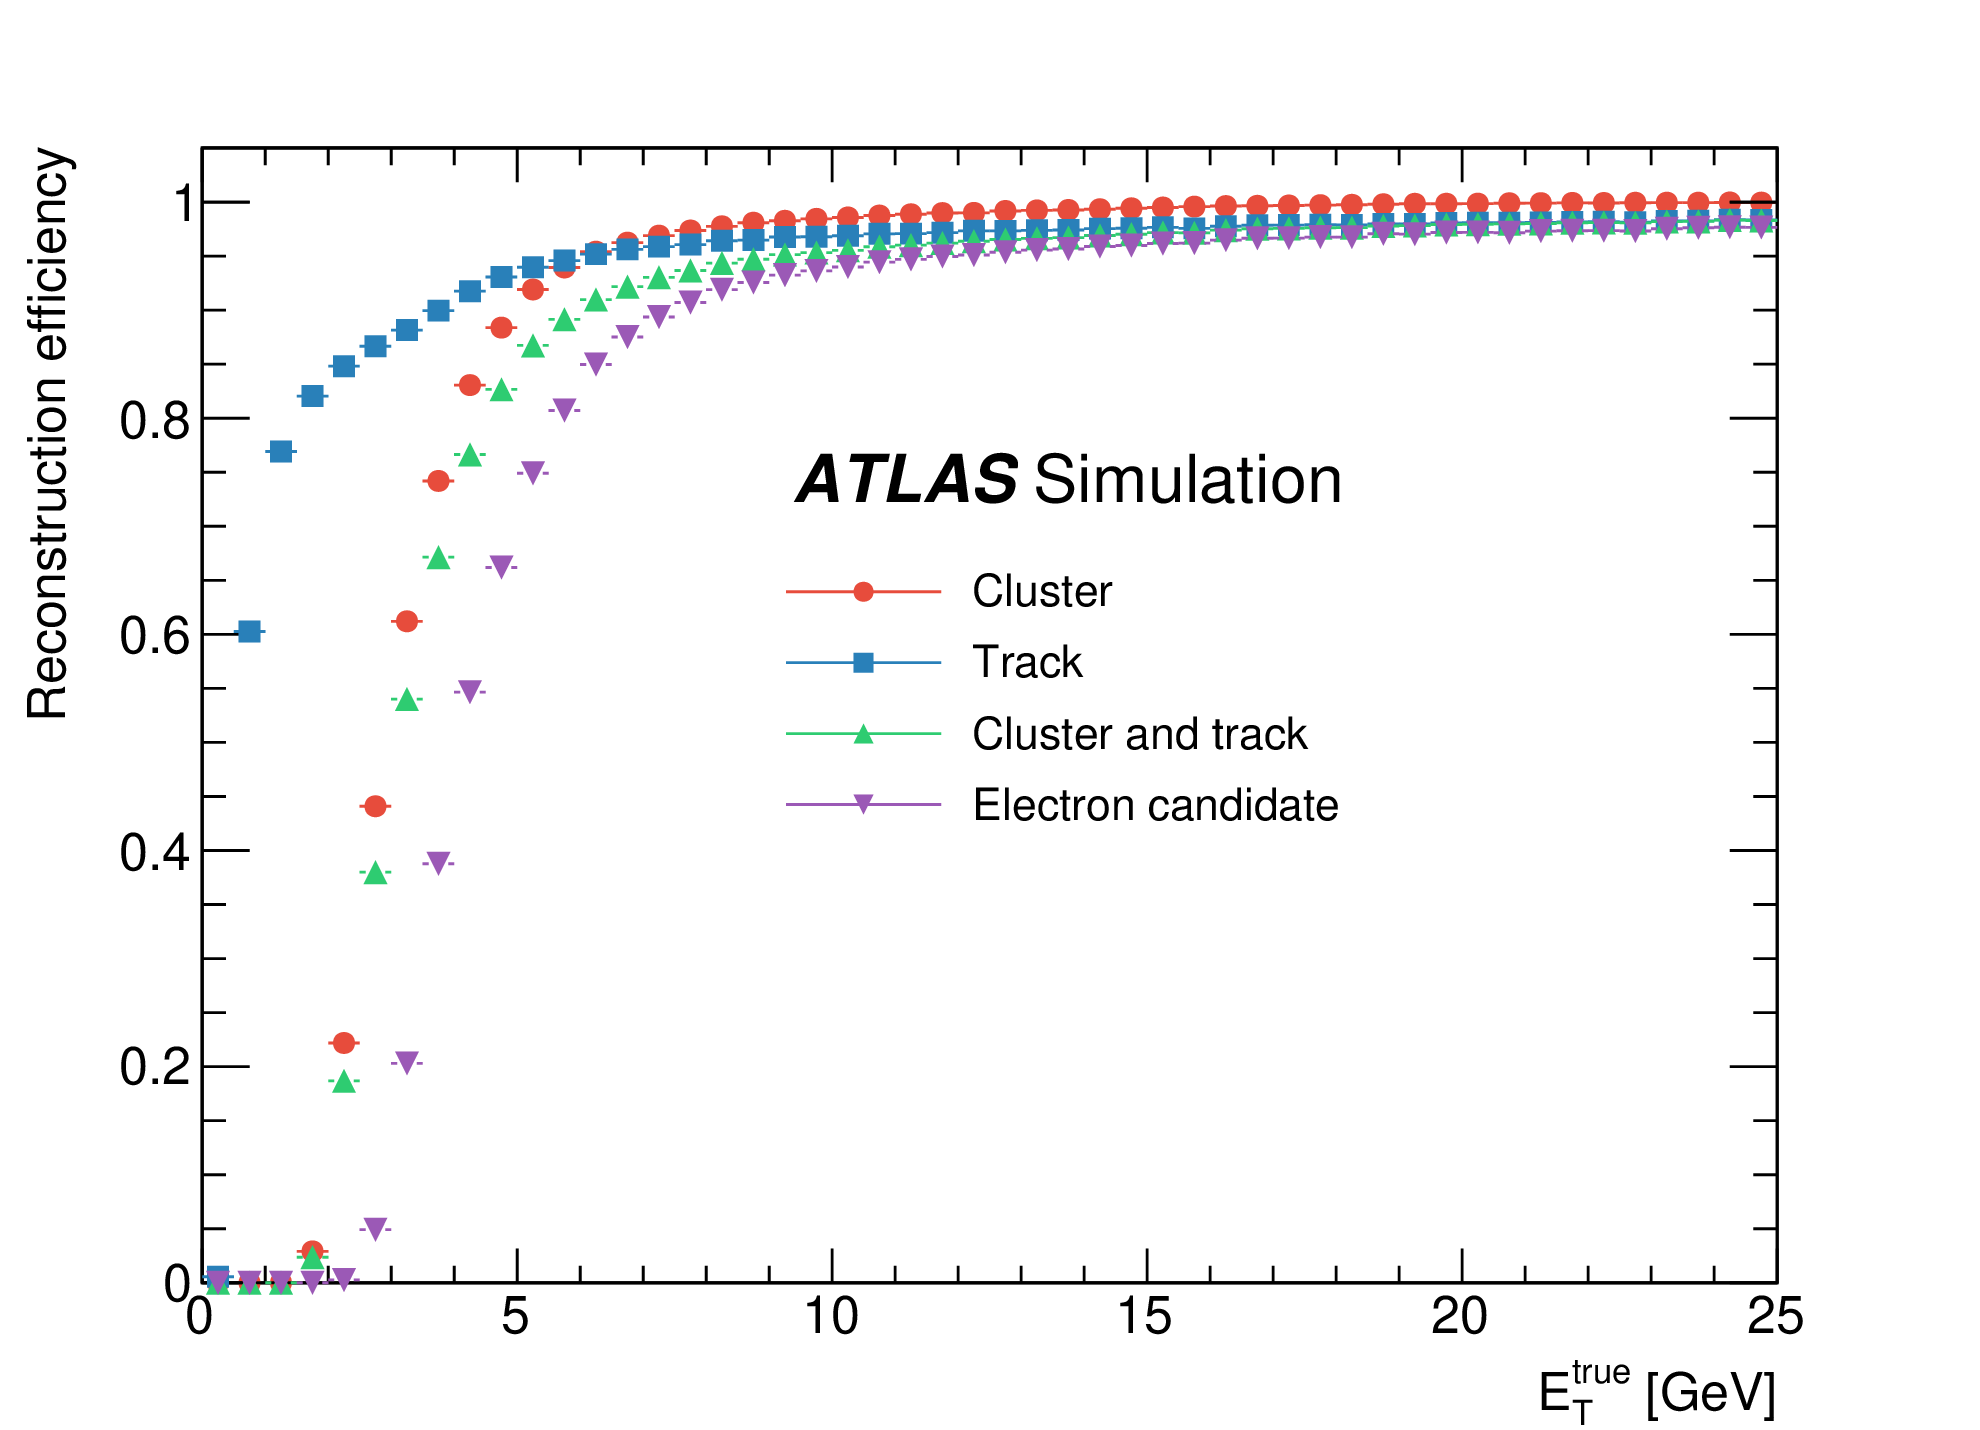
\includegraphics[width=\mediumfigwidth]{images/supercluster_reco.png}
    \caption[Supercluster based cluster, track, cluster and track, and electron reconstruction efficiencies as a function of the generated electron $E_T$ ]{Supercluster based cluster, track, cluster and track, and electron reconstruction efficiencies as a function of the generated electron $E_T$~\cite{Aad:2019tso}.}
    \label{fig:method:screco}
\end{figure}

The supercluster based algorithm provides an improved energy resolution compared to the sliding window algorithm by collecting more energy deposits. The peak energy response $E_{calib}/E_{true}$ does not deviate by more than 0.5\% for the different particles, where $E_{true}$ is the energy of the particles prior to detector simulation and $E_{calib}$ is the calibrated reconstructed energy. The \emph{effective interquartile range} (IQE) compares the width (resolution) of the energy response, and can be used to quantify the performance supercluster algorithm compared to the sliding window algorithm. 
\begin{equation}
    IQE = \frac{Q_3 - Q_1}{1.349},
\end{equation}
where $Q_1$ and $Q_3$ are the first and third quartiles of the $E_{calib}/E_{true}$ distribution, and a normalisation factor chosen such that the IQE of a Gaussian distribution equals it's standard deviation. The supercluster algorithm shows a significant improvement in the resolution for electrons compared to the sliding window algorithm. \cref{fig:method:iqe} shown the IQE as a function of energy is shown for the two approaches. 
\begin{figure}[h]
    \centering
    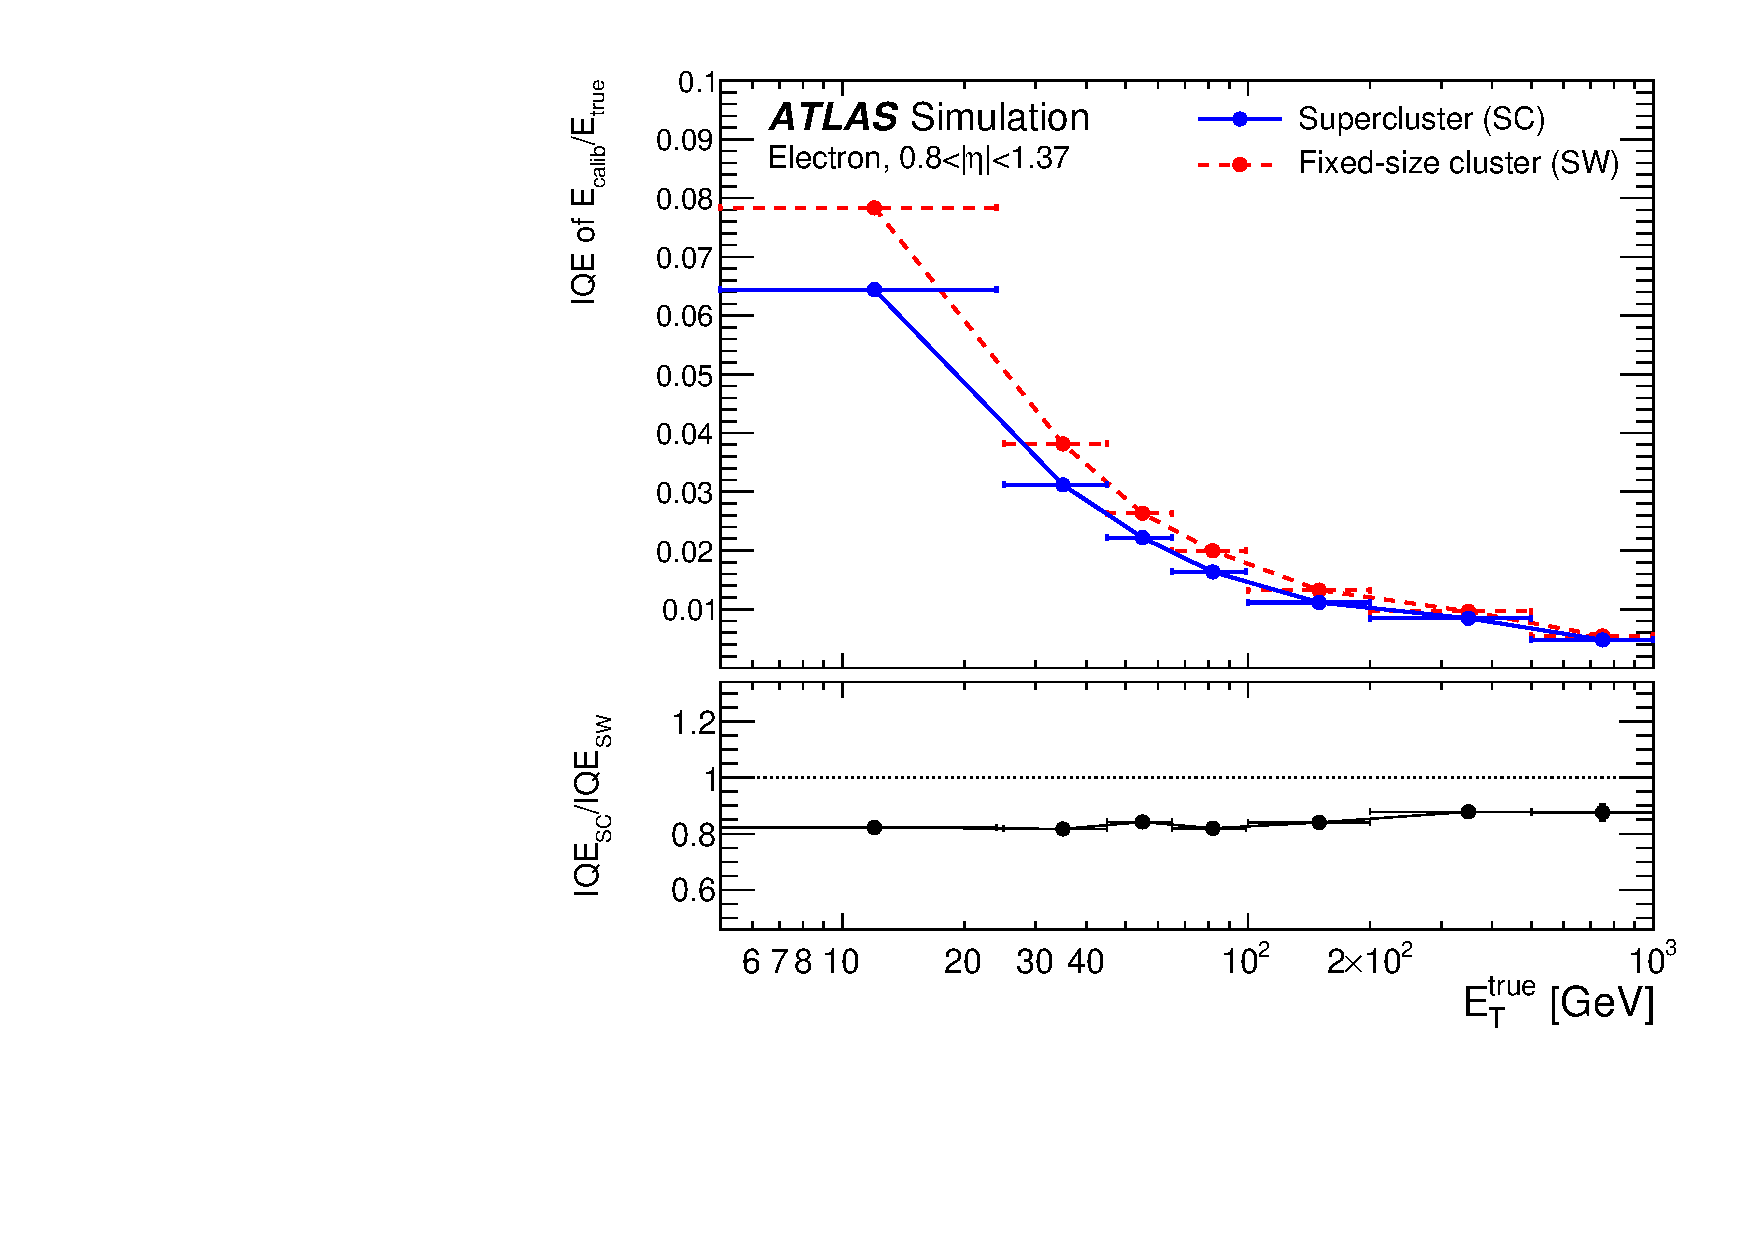
\includegraphics[width=\mediumfigwidth]{images/IQE_reco_1.pdf}
    \caption[Calibrated energy response resolution, expressed in terms of IQE, for simulated electrons]{Calibrated energy response resolution, expressed in terms of IQE, for simulated electrons .The response for fixed-size clusters based on the sliding window method is shown in dashed red, while the supercluster-based one is shown in full blue~\cite{Aad:2019tso}.}
    \label{fig:method:iqe}
\end{figure}

\subsubsection{Electron idendtification}
A large proportion of reconstructed electron candidates may not be real electrons. It is possible for a physics processes to fake the prompt electron signature. Prompt electrons are defined as electrons which come from the hard scattering vertex and are not the result of hadronic decays. Fake prompt electrons can arise from source such as, hadronic showers which mimic an electron shower, electrons from photon conversions and, the semileptonic decays of heavy flavour hadrons.

Therefore, further criteria, referred to as \emph{identification} is defined to select a sample of pure prompt electrons. A likelihood based identification method is used in the identification of prompt electrons. The method combined 

\subsection{Event Generation}

\subsection{Detector Simulation}

\subsection{Full Simulation}

\subsection{ATLAS Fast Simulation}


